\documentclass[12pt, a4paper]{article}

% ==========================================
% 1. KHAI BÁO GÓI THƯ VIỆN (PACKAGES)
% ==========================================
% Bảng mã & Font chữ
\usepackage[utf8]{inputenc}
\usepackage[T5]{fontenc}

% Toán học
\usepackage{amsmath, amssymb}

% Căn lề & Bố cục trang
\usepackage[top=2.2cm, bottom=1.5cm, left=1cm, right=1cm, headheight=15pt]{geometry}
\usepackage{fancyhdr}
\usepackage{needspace}
\usepackage{tkz-tab}

% Đồ họa & Màu sắc
\usepackage{xcolor}
\usepackage{graphicx} 
\usepackage{tikz}
\usetikzlibrary{calc, shapes.geometric, positioning}


% Bảng biểu & Danh sách
\usepackage{colortbl}
\usepackage{array}
\usepackage{makecell}
\usepackage{multirow}
\usepackage{tasks}

% Biểu tượng
\usepackage{fontawesome5}

% ==========================================
% 2. THIẾT LẬP MÀU SẮC CHỦ ĐẠO
% ==========================================
\definecolor{goldyellow}{RGB}{255, 179, 0}
\definecolor{amberorange}{RGB}{230, 115, 0}
\definecolor{lightamber}{RGB}{255, 248, 225}
\definecolor{deepblue}{RGB}{25, 42, 86}
\definecolor{accentred}{RGB}{232, 65, 24}
\definecolor{softgray}{RGB}{220, 220, 222} 
\definecolor{fbblue}{RGB}{15, 80, 200}


% ==========================================
% 3. CẤU HÌNH HEADER & FOOTER
% ==========================================
\pagestyle{fancy}
\fancyhf{}
\renewcommand{\headrulewidth}{0pt}

% Khai báo biến lưu trữ nội dung góc phải của Header
\newcommand{\HeaderRightText}{}

% --- Header ---
\fancyhead[C]{
    \begin{tikzpicture}[remember picture, overlay]
        
        % Dải màu trang trí góc trên
        \path[fill=deepblue] (current page.north west) -- (current page.north east) 
            -- ($(current page.north east) + (0, -1.6cm)$) 
            .. controls ($(current page.north) + (3, -2.0cm)$) and ($(current page.north) + (-3, -0.4cm)$) .. 
            ($(current page.north west) + (0, -1.0cm)$) -- cycle;
            
        \path[fill=goldyellow] (current page.north west) -- (current page.north east) 
            -- ($(current page.north east) + (0, -1.0cm)$) 
            .. controls ($(current page.north) + (4, -1.0cm)$) and ($(current page.north) + (-2, -2.2cm)$) .. 
            ($(current page.north west) + (0, -1.6cm)$) -- cycle;
            
        \path[fill=amberorange] (current page.north west) -- ($(current page.north west) + (6.5cm, 0)$) 
            .. controls ($(current page.north west) + (4.5cm, -1.2cm)$) and ($(current page.north west) + (2cm, -2.0cm)$) .. 
            ($(current page.north west) + (0, -2.0cm)$) -- cycle;
            
        % Logo góc trái Header
        \node[anchor=west, inner sep=0pt] 
            at ($(current page.north west) + (0cm, -0.8cm)$) {
\includegraphics[height=2.0cm]{../../../image/logo-header.png}};
            
        % Text góc phải Header (Tự động lấy từ đối số thứ 3 của \titlebox)
        \node[anchor=east, text=white, font=\small\bfseries\sffamily] 
            at ($(current page.north east) + (-0.8cm, -0.5cm)$) {\HeaderRightText};
    \end{tikzpicture}
}

% --- Footer ---
\fancyfoot[C]{
    \begin{tikzpicture}[remember picture, overlay]
        % Đường kẻ ngang
        \draw[amberorange, line width=1.5pt] 
            ($(current page.south west) + (0cm, 0.4cm)$) -- ($(current page.south east) + (0cm, 0.4cm)$);

        % Dải cong góc phải
        \path[fill=goldyellow] (current page.south east) -- ($(current page.south east) + (-5cm, 0)$) 
            .. controls ($(current page.south east) + (-3cm, 0.8cm)$) and ($(current page.south east) + (-1.5cm, 1.2cm)$) .. 
            ($(current page.south east) + (0, 1.2cm)$) -- cycle;

        % Mạng xã hội
        \node[anchor=west, inner sep=0pt] at ($(current page.south west) + (1cm, 0.8cm)$) {
            \small\sffamily
            \textcolor{fbblue}{\faFacebook\hskip 4pt Toán Anh Huy MATH-STER}
            \hskip 18pt
            \textcolor{black}{\faTiktok\hskip 4pt huymathster}
        };

        % Số trang (Thiết kế hình tròn cũ thu nhỏ)
        \node[circle, fill=white, draw=amberorange, line width=1.5pt, text=deepblue, font=\large\bfseries, inner sep=0pt, minimum size=0.7cm] 
            at ($(current page.south east) + (-1.0cm, 0.65cm)$) {\thepage};
    \end{tikzpicture}
}

% ==========================================
% 4. ĐỊNH NGHĨA MACRO: KHUNG TIÊU ĐỀ
% ==========================================
\newcommand{\titlebox}[3]{
    % Gán nội dung đối số #3 vào biến HeaderRightText
    \gdef\HeaderRightText{#3}
    
    \begin{center}
    \vspace*{-0.5cm}
    \begin{tikzpicture}
        % Khung vô hình (Phantom Box) định chuẩn kích thước
        \node[text width=16cm, inner xsep=0pt, inner ysep=16pt, opacity=0] (MainBox) {
            \begin{minipage}[c]{4.2cm}
                \centering\vspace{0.1cm}
                \rule{2.2cm}{2.2cm} 
                \vspace{0.1cm}
            \end{minipage}%
            \begin{minipage}[c]{11.5cm}
                \centering\vspace{0.15cm}
                {\huge\bfseries\sffamily #2 \par}
                \vspace{0.15cm} 
            \end{minipage}
        };
        
        % Đổ bóng & Nền
        \fill[goldyellow, rounded corners=8pt] ([xshift=5pt, yshift=-5pt]MainBox.south west) rectangle ([xshift=5pt, yshift=-5pt]MainBox.north east);
        \fill[white, rounded corners=8pt] (MainBox.south west) rectangle (MainBox.north east);
        
        % Lưới ô ly & Nền Logo
        \begin{scope}
            \clip[rounded corners=8pt] (MainBox.south west) rectangle (MainBox.north east);
            \draw[step=0.4cm, softgray!50, line width=0.6pt] (MainBox.south west) grid (MainBox.north east);
            \fill[lightamber!60] (MainBox.south west) rectangle ([xshift=4.2cm]MainBox.north west);
        \end{scope}

        % Viền ngoài
        \draw[deepblue, line width=1.5pt, rounded corners=8pt] (MainBox.south west) rectangle (MainBox.north east);

        % Nội dung Text (Lớp trên cùng)
        \node[text width=16cm, inner xsep=0pt, inner ysep=16pt] at (MainBox.center) {
            \begin{minipage}[c]{4.2cm}
                \centering
                % --- ĐIỀU CHỈNH TỌA ĐỘ LOGO Ở ĐÂY ---
                \hspace*{-0.5cm}\raisebox{-0.2cm}{
\includegraphics[width=5.5cm]{../../../image/logo.png}}
            \end{minipage}%
            \begin{minipage}[c]{11.5cm}
                \centering\vspace{0.15cm}
                {\huge\bfseries\sffamily\color{deepblue} #2 \par}
                \vspace{0.15cm} 
            \end{minipage}
        };
        
        % Trang trí phụ kiện
        \draw[deepblue, line width=1.5pt, dashed] ([xshift=4.2cm]MainBox.north west) -- ([xshift=4.2cm]MainBox.south west);
        \node[regular polygon, regular polygon sides=4, rotate=45, fill=white, draw=accentred, line width=1.2pt, inner sep=2.5pt] at ([xshift=4.2cm]MainBox.west) {};
        \node[anchor=west, fill=amberorange, text=white, font=\large\bfseries\sffamily, rounded corners=4pt, draw=deepblue, line width=1.5pt, inner xsep=12pt, inner ysep=6pt] at ([xshift=1.5cm]MainBox.north west) {#1};
        \fill[accentred] ([xshift=-1.8cm, yshift=-0.4cm]MainBox.north east) circle (3pt);
        \fill[amberorange] ([xshift=-1.4cm, yshift=-0.4cm]MainBox.north east) circle (3pt);
        \fill[goldyellow] ([xshift=-1.0cm, yshift=-0.4cm]MainBox.north east) circle (3pt);
    \end{tikzpicture}
    \vspace*{0cm}
    \end{center}
}

% ==========================================
% 5. ĐỊNH NGHĨA MACRO: CẤU TRÚC CÂU HỎI (ÉP SÁT NHAU)
% ==========================================
\newcommand{\questioncore}[2]{
    % Xóa khoảng cách phía trên, ép sát câu trước
    \noindent \textbf{\textcolor{deepblue}{Câu #1.} \textcolor{accentred}{[STER]}} #2
    \par\nopagebreak
}

% Cấu hình hiển thị đáp án trắc nghiệm
\settasks{
    label=\textbf{\textcolor{amberorange}{\Alph*.}}, 
    label-width=15pt,     
    item-indent=25pt,     
    label-offset=6pt,    
    column-sep=20pt,     
    after-item-skip=2pt  % Đã giảm tối đa khoảng cách giữa các dòng đáp án A B C D
}

% Hàm vẽ dòng kẻ nháp
\newcommand{\drawdashlines}[1]{
    \ifnum#1>0
        \nopagebreak\vspace{0.1cm}\noindent 
        \begin{tikzpicture}
            \foreach \i in {1,...,#1} {
                \draw[softgray, line width=0.2pt] (0,-{\i*0.8}) -- (\textwidth-4pt,-{\i*0.8});
            }
        \end{tikzpicture}
        \par
    \fi
    % Đã xóa hoàn toàn khoảng cách thừa ở nhánh else
}

% --- Dạng 1: Trắc nghiệm 4 đáp án ---
\newcommand{\questionLinesManual}[4]{
    \pgfmathsetmacro{\calculatedSpace}{1.5 + #1 * 0.65}
    \needspace{\calculatedSpace cm} 
    \questioncore{#2}{#3}
    #4
    \par\nopagebreak
    \drawdashlines{#1}
}

\usepackage{cellspace}
\setlength\cellspacetoplimit{4pt}    % Khoảng đệm tự động phía trên ô
\setlength\cellspacebottomlimit{4pt} % Khoảng đệm tự động phía dưới ô




\newcommand{\questionTrueFalse}[4]{
    \pgfmathsetmacro{\calculatedSpace}{3.0 + #1 * 0.65} 
    \needspace{\calculatedSpace cm}
    \questioncore{#2}{#3}
    
    \nopagebreak
    \begin{center}
    \begin{tabular}{|>{\centering\arraybackslash}S{m{0.8cm}}|S{m{12cm}}|>{\centering\arraybackslash}S{m{1.5cm}}|>{\centering\arraybackslash}S{m{1.5cm}}|}
        \hline
        \rowcolor{amberorange!20}
        \multicolumn{1}{|c|}{} & \multicolumn{1}{>{\centering\arraybackslash}m{12cm}|}{\textbf{\textcolor{deepblue}{Mệnh đề}}} & 
        \textbf{\textcolor{deepblue}{Đúng}} & 
        \textbf{\textcolor{deepblue}{Sai}} \\
        \hline
        #4
        \hline
    \end{tabular}
    \end{center}
    
    \par\nopagebreak
    \drawdashlines{#1}
}

% ----- Dạng 3: Tự luận ngắn -----
\newcommand{\questionShortAnswer}[3]{
    \pgfmathsetmacro{\calculatedSpace}{1.5 + #1 * 0.8}
    \needspace{\calculatedSpace cm}
    
    {\linespread{1.1}\selectfont % Bóp nhỏ giãn dòng của câu tự luận
    \questioncore{#2}{#3}\par}
    
    \nopagebreak
    \begin{flushright}
        \begin{tikzpicture}
            \node[anchor=east, font=\small\bfseries\sffamily, text=deepblue] 
                at (-0.2, 0.4) {Đáp án:};
            \fill[goldyellow, rounded corners=3pt] (0.08, -0.08) rectangle (3.08, 0.72);
            \draw[draw=deepblue, fill=white, line width=1.2pt, rounded corners=3pt] 
                (0,0) rectangle (3.0, 0.8);
            \foreach \x in {0.75, 1.5, 2.25} {
                \draw[draw=deepblue, line width=0.6pt] (\x, 0) -- (\x, 0.8);
            }
        \end{tikzpicture}
    \end{flushright}
    
    \par\nopagebreak
    \drawdashlines{#1}
}


\settasks{
    after-item-skip = 1em % Tương đương row-skip cũ
}

% ==========================================
% BẮT ĐẦU NỘI DUNG TÀI LIỆU
% ==========================================
\begin{document}

% Truyền 3 tham số: {Nhãn cam} {Chữ to chính giữa} {Chữ ở góc phải Header}
\titlebox{Chủ đề: Tích phân}{Ứng dung tích phân tính diện tích thể tính}{Nguyên hàm - Tích phân: Ứng dụng}

% --- CÂU 1 ---
\questionLinesManual{0}{1}{Diện tích hình phẳng giới hạn bởi đồ thị hàm số \( y = x^3 - 4x \), trục hoành và hai đường thẳng \( x = 0 \), \( x = 3 \) bằng:}{%
    \begin{tasks}(4)
        \task \( \displaystyle\int_{0}^{3} |x^3 - 4x| dx \)
        \task \( \displaystyle\pi \int_{0}^{3} |x^3 - 4x| dx \)
        \task \( \displaystyle\pi \int_{0}^{3} (x^3 - 4x)^2 dx \)
        \task \( \displaystyle\int_{0}^{3} (x^3 - 4x) dx \)
    \end{tasks}
}

% --- CÂU 2 ---
\questionLinesManual{0}{2}{Diện tích \( S \) của hình phẳng giới hạn bởi các đường \( y = 3x^2 \), \( y = -2 \), \( x = 0 \) và \( x = 1 \) được tính bởi công thức nào sau đây?}{%
    \begin{tasks}(4)
        \task \( \displaystyle\int_{0}^{1} (3x^2 + 2) dx \)
        \task \( \displaystyle\int_{0}^{1} |3x^2 - 2| dx \)
        \task \( \displaystyle\pi \int_{0}^{1} (3x^2 + 2)^2 dx \)
        \task \( \displaystyle\pi \int_{0}^{1} (3x^2 + 1)^2 dx \)
    \end{tasks}
}

% --- CÂU 3 ---
\questionLinesManual{0}{3}{Cho hình phẳng \( (H) \) giới hạn bởi đồ thị \( y = 2x - x^2 \) và trục hoành. Thể tích vật thể tròn xoay sinh ra khi cho \( (H) \) quay quanh trục hoành bằng}{%
    \begin{tasks}(4)
        \task \( \dfrac{16}{15} \)
        \task \( \dfrac{4}{3} \)
        \task \( \dfrac{16\pi}{15} \)
        \task \( \dfrac{4\pi}{3} \)
    \end{tasks}
}

% --- CÂU 4 ---
\questionLinesManual{0}{4}{Tính thể tích \( V \) của phần vật thể giới hạn bởi hai mặt phẳng \( x = 0, x = 1 \), có thiết diện bị cắt bởi mặt phẳng vuông góc với trục \( Ox \) tại điểm có hoành độ \( x(0 \leq x \leq 1) \) là một tam giác đều có cạnh bằng \( x \).}{%
    \begin{tasks}(4)
        \task \( V = \dfrac{12\pi}{5} \)
        \task \( V = \dfrac{12}{5} \)
        \task \( V = \dfrac{\sqrt{3}\pi}{12} \)
        \task \( V = \dfrac{\sqrt{3}}{12} \)
    \end{tasks}
}

% --- CÂU 5 ---
\questionLinesManual{0}{5}{Cho hình phẳng \( (H) \) giới hạn bởi các đường  
\( y = x^2 + 3, \, y = 0, \, x = 0, \, x = 2. \)  
Gọi \( V \) là thể tích khối tròn xoay được tạo thành khi quay \( (H) \) xuống quanh trục \( Ox \). Mệnh đề nào sau đây đúng?}{%
    \begin{tasks}(4)
        \task \( \displaystyle V = \pi \int_{0}^{2} (x^2 + 3) dx \)
        \task \( \displaystyle V = \int_{0}^{2} (x^2 + 3) dx \)
        \task \( \displaystyle V = \pi \int_{0}^{2} (x^2 + 3)^2 dx \)
        \task \( \displaystyle V = \int_{0}^{2} (x^2 + 3)^2 dx \)
    \end{tasks}
}

% --- CÂU 6 ---
\questionLinesManual{0}{6}{Diện tích của hình phẳng được tô màu trong hình bên dưới được tính theo công thức nào?

\begin{center}
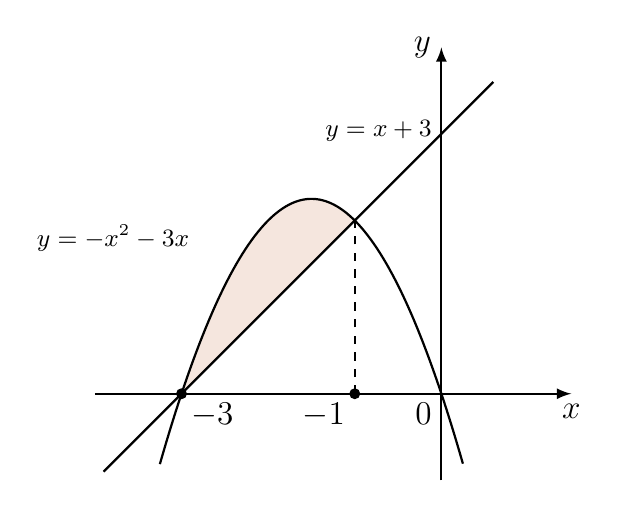
\begin{tikzpicture}[>=latex, scale=1.1]
    % Định nghĩa màu tô cho miền giới hạn (màu nâu/cam nhạt)
    \definecolor{fillcolor}{RGB}{245, 230, 222}
    \definecolor{brownline}{RGB}{139, 69, 19}

    % 1. Tô màu miền giới hạn giữa Parabola và Đường thẳng
    \fill[fillcolor] 
        plot[domain=-3:-1, samples=100] (\x, {-\x*\x - 3*\x}) -- 
        plot[domain=-1:-3, samples=100] (\x, {\x + 3}) -- cycle;

    % 2. Trục tọa độ
    \draw[->, thick] (-4.0,0) -- (1.5,0) node[below] {\large $x$};
    \draw[->, thick] (0,-1) -- (0,4) node[left] {\large $y$};

    % 3. Đồ thị các hàm số
    % Parabola y = -x^2 - 3x (Phần trong miền tô màu làm đậm màu nâu)
    \draw[thick, samples=100, domain=-3.25:0.25] 
        plot (\x, {-\x*\x - 3*\x});
    \node[left] at (-2.8, 1.8) {\small $y = -x^2 - 3x$};

    % Đường thẳng y = x + 3
    \draw[thick, domain=-3.9:0.6] 
        plot (\x, {\x + 3});
    
    \node[above left] at (0, 2.8) {\small $y = x + 3$};

    % 4. Đường gióng nét đứt và điểm giao
    \draw[dashed, thick] (-1,0) -- (-1,2);

    \fill (-3,0) circle (1.8pt) node[below right] {\large $-3$};
    \fill (-1,0) circle (1.8pt) node[below left] {\large $-1$};
    \node[below left] at (0,0) {\large $0$};
\end{tikzpicture}
\end{center}
}{%
    \begin{tasks}(4)
        \task \( \displaystyle\int_{-3}^{-1} (-x^2 - 4x - 3) dx \)
        \task \( \displaystyle\int_{-3}^{-1} (x^2 + 4x - 3) dx \)
        \task \( \displaystyle\int_{-3}^{-1} (-x^2 - 4x + 3) dx \)
        \task \( \displaystyle\int_{-3}^{-1} (x^2 + 4x + 3) dx \)
    \end{tasks}
}

% --- CÂU 7 ---
\questionLinesManual{0}{7}{Cho hình phẳng \( (H) \) giới hạn bởi các đường \( y = x^2 - 2x - 1 \), \( y = 2x - 4 \). Diện tích hình phẳng giới hạn bởi hình \( (H) \) bằng}{%
    \begin{tasks}(4)
        \task \( \dfrac{2}{3} \)
        \task \( \dfrac{4}{3} \)
        \task \( \dfrac{8}{3} \)
        \task 4
    \end{tasks}
}

% --- CÂU 8 ---
\questionLinesManual{0}{8}{Cho hàm số \( y = f(x) \). Biết rằng phần hình phẳng giới hạn bởi \( S_1 \) và \( S_2 \) (xem hình vẽ dưới đây) có diện tích lần lượt bằng 7 và 2. Tích phân \(\displaystyle\int_{-1}^{4} f(x) dx\) bằng

\begin{center}
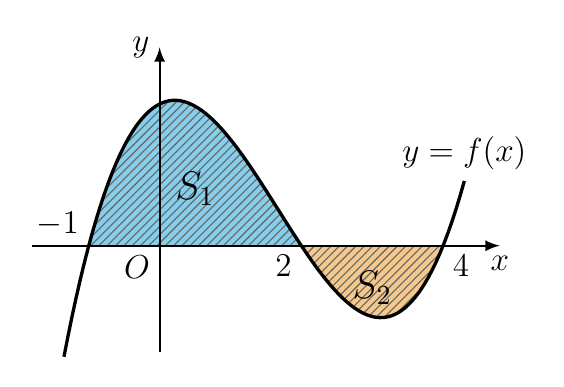
\begin{tikzpicture}[>=latex, scale=0.9]
    % Thư viện cần dùng: \usetikzlibrary{patterns}

    % Định nghĩa màu sắc cho hai miền
    \definecolor{cyanfill}{RGB}{135, 206, 235}  % Màu xanh lam nhạt cho S1
    \definecolor{orangefill}{RGB}{245, 200, 140} % Màu cam nhạt cho S2

    % 1. Tô nền và gạch chéo cho miền S1 (từ x = -1 đến x = 2)
    \fill[cyanfill] 
        plot[domain=-1:2, samples=100] (\x, {0.25*(\x+1)*(\x-2)*(\x-4)}) -- 
        (2,0) -- (-1,0) -- cycle;
    \fill[pattern=north east lines, pattern color=black!60] 
        plot[domain=-1:2, samples=100] (\x, {0.25*(\x+1)*(\x-2)*(\x-4)}) -- 
        (2,0) -- (-1,0) -- cycle;

    % 2. Tô nền và gạch chéo cho miền S2 (từ x = 2 đến x = 4)
    \fill[orangefill] 
        plot[domain=2:4, samples=100] (\x, {0.25*(\x+1)*(\x-2)*(\x-4)}) -- 
        (4,0) -- (2,0) -- cycle;
    \fill[pattern=north east lines, pattern color=black!60] 
        plot[domain=2:4, samples=100] (\x, {0.25*(\x+1)*(\x-2)*(\x-4)}) -- 
        (4,0) -- (2,0) -- cycle;

    % 3. Trục tọa độ
    \draw[->, thick] (-1.8,0) -- (4.8,0) node[below] {\large $x$};
    \draw[->, thick] (0,-1.5) -- (0,2.8) node[left] {\large $y$};
    \node[below left] at (0,0) {\large $O$};

    % 4. Đồ thị hàm số y = f(x)
    \draw[very thick, samples=100, domain=-1.35:4.3] 
        plot (\x, {0.25*(\x+1)*(\x-2)*(\x-4)}) 
        node[above] {\large $y = f(x)$};

    % 5. Nhãn miền S1, S2 và các mốc tọa độ
    \node at (0.5, 0.8) {\Large $S_1$};
    \node at (3.0, -0.6) {\Large $S_2$};

    \node[above left] at (-1,0) {\large $-1$};
    \node[below left] at (2,0) {\large $2$};
    \node[below right] at (4,0) {\large $4$};
\end{tikzpicture}
\end{center}
}{%
    \begin{tasks}(4)
        \task 9
        \task -5
        \task -9
        \task 5
    \end{tasks}
}

% --- CÂU 9 ---
\questionLinesManual{0}{9}{Cho hàm số \( y = f(x) \) có đồ thị như Hình. Gọi \( S \) là phần diện tích hình phẳng được tô màu. Phát biểu nào sau đây là đúng?

\begin{center}
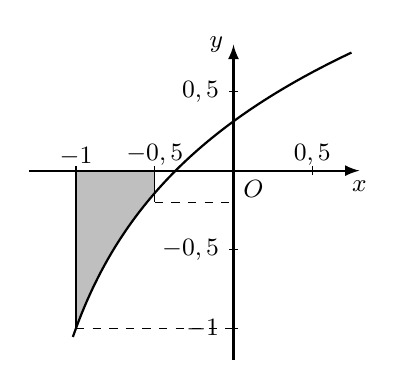
\begin{tikzpicture}[>=latex, scale=2.0]
    % 1. Tô màu xám miền giới hạn (từ x = -1 đến x = -0.5)
    % Hàm số phác họa: y = ln(x + 1.368)
    \fill[gray!50] 
        plot[domain=-1:-0.5, samples=100] (\x, {ln(\x + 1.367879)}) -- 
        (-0.5,0) -- (-1,0) -- cycle;

    % 2. Trục tọa độ
    \draw[->, thick] (-1.3,0) -- (0.8,0) node[below] {\small $x$};
    \draw[->, thick] (0,-1.2) -- (0,0.8) node[left] {\small $y$};
    \node[below right] at (0,0) {\small $O$};

    % 3. Đánh dấu các mốc tọa độ
    % Trục Ox
    \draw (-1,0.03) -- (-1,-0.03) node[above] {\small $-1$};
    \draw (-0.5,0.03) -- (-0.5,-0.03) node[above] {\small $-0,5$};
    \draw (0.5,0.03) -- (0.5,-0.03) node[above] {\small $0,5$};

    % Trục Oy
    \draw (0.03,-1) -- (-0.03,-1) node[left] {\small $-1$};
    \draw (0.03,-0.5) -- (-0.03,-0.5) node[left] {\small $-0,5$};
    \draw (0.03,0.5) -- (-0.03,0.5) node[left] {\small $0,5$};

    % 4. Đồ thị hàm số
    \draw[thick, samples=100, domain=-1.02:0.75] 
        plot (\x, {ln(\x + 1.367879)});

    % 5. Các đường gióng nét đứt và nét liền
    \draw[dashed] (-1,-1) -- (0,-1);
    \draw[dashed] (-0.5,-0.2) -- (0,-0.2);
    
    % Đường đứng ranh giới tại x = -1 và x = -0.5
    \draw (-1,0) -- (-1,-1);
    \draw (-0.5,0) -- (-0.5,-0.2);
\end{tikzpicture}
\end{center}
}{%
    \begin{tasks}(4)
        \task \( S = \displaystyle\int_{-1}^{0} f(x) dx \)
        \task \( S = -\displaystyle\int_{-1}^{0} f(x) dx \)
        \task \( S = -\left| \displaystyle\int_{-1}^{0} f(x) dx \right| \)
        \task \( S = -\displaystyle\int_{-1}^{0} f(x) dx \)
    \end{tasks}
}

% --- CÂU 10 ---
\questionLinesManual{0}{10}{Tính diện tích hình phẳng giới hạn bởi đồ thị hàm số \( y = e^x \), trục hoành và hai đường thẳng  
\( x = 0 \) và \( x = 3 \).}{%
    \begin{tasks}(4)
        \task \( e^3 \)
        \task \( e^3 - 1 \)
        \task \( e^2 - 1 \)
        \task \( e(e^2 - 1) \)
    \end{tasks}
}

\end{document}
